\section{Introduction}
\label{sec:intro}
\textcolor{red}{TODO: (1) Survey Comparison table (with other surveys and perspectives.) (2) Modify the intro and structures (3) keep refining the figures
% Motivation:
% (1) inference-time optimization as a behavioral governance problem rather than purely a performance one
% (2) trustworthiness surveys mention inference-time ideas, but treat them individually (prompting, decoding, guardrails) rather than as a coherent design space.
% (3) Complementary to other surveys. (Maybe after RLHF, more dynamic)


% Large Language Models (LLMs) have moved from research prototypes to widely deployed decision-support systems in domains such as healthcare, finance, and law. Built on massive neural architectures and web-scale corpora, they exhibit strong abilities in language understanding, generation, and multi-step reasoning. 
% However, their expanding societal integration introduces trustworthy issues such that models can generate harmful or biased content, leak sensitive information, or hallucinate plausible but false claims. We leverage \emph{trustworthiness} to denote reliability at deployment along four axes: safety, privacy, fairness, and factuality. Ensuring these properties requires not only capable models but also robust mechanisms for \emph{behavioral control at inference time}.

% Training-time alignment (e.g., instruction tuning and Reinforcement Learning from Human Feedback, RLHF) sets broad behavioral priors by updating model parameters. These methods are essential for transforming base models into helpful and safe assistants. Yet they are inherently static: once trained, behavior is costly to change; access to weights may be limited (API-only); and new policies, users, or contexts emerge faster than retraining cycles. We argue that \emph{inference-time methods} constitute a necessary \emph{control plane} for trustworthy deployment. They provide agile, modular, and cost-effective levers for adaptation. These methods can range from interventions on black-box models to lightweight parameter modifications, but all enable rapid adaptation \emph{without} the high cost and latency of full model retraining. The goal is not to replace training-time alignment but to complement it as part of a defense-in-depth design.

% Research into inference-time methods is not new. Traditionally, such techniques have been employed to shape model generation toward various goals, including improving output quality (e.g., coherence or factual grounding via retrieval) and optimizing computational efficiency (e.g., latency and memory). However, the widespread deployment of LLMs in high-stakes domains has elevated the use of these techniques for a distinct and critical purpose: serving as a behavioral control layer for trustworthiness.

% This role is complementary to, yet distinct from, training-time alignment (e.g., RLHF). While training-time methods are vital for establishing broad, static behavioral priors, they are inherently ill-suited for the dynamic and context-specific demands of live deployment. Deployed systems face rapidly evolving constraints that static, pre-trained models cannot address alone: organizations increasingly need to (i) update safety or content policies instantly, far faster than any retraining cycle permits; (ii) personalize behavioral rules for specific users, contexts, or jurisdictions; (iii) provide auditable interventions (e.g., redaction) for regulatory compliance; and (iv) respond immediately to newly discovered vulnerabilities, distribution shifts, or jailbreak attacks. Therefore, this paper focuses on inference-time control as the critical and agile plane for enforcing these dynamic trustworthiness constraints. It is the necessary counterpart to static training-time alignment, enabling reliable operation in real-world environments.

% To structure our analysis, we focus on four core dimensions of trustworthiness:

% \begin{itemize}
%     \item \textbf{Safety:} Prevent harmful, toxic, biased, or malicious content; mitigate misuse (e.g., disinformation); defend against \emph{jailbreak} and \emph{backdoor} attacks.
%     \item \textbf{Privacy:} Avoid memorization and leakage of sensitive data from pre-training corpora; protect the confidentiality of user inputs at inference.
%     \item \textbf{Fairness:} Reduce systematic disadvantages to individuals or groups on the basis of protected attributes.
%     \item \textbf{Factuality:} Ground outputs in verifiable evidence and established world knowledge, minimizing hallucinations.
% \end{itemize}

% We define inference-time methods as post-training interventions that guide, constrain, or steer model behavior during or immediately around generation, without full retraining. These techniques span a spectrum from purely black-box controls on inputs/outputs (e.g., prompting, guardrails, decoding) to lightweight but more intrusive interventions on activations or parameters (e.g., representation steering, editing, unlearning, pruning). Some approaches incorporate auxiliary modules (e.g., compact classifiers or retrieval), yet the primary LLM weights remain unchanged.

% To provide a structured overview of this landscape, we propose a unified taxonomy of eight categories: \textbf{Context Engineering}, \textbf{Guardrails}, \textbf{Decoding Strategies}, \textbf{Representation Engineering}, \textbf{Editing}, \textbf{Unlearning}, \textbf{Pruning}, and \textbf{Multi-Agent Systems}. The purpose of this taxonomy is to frame these techniques not as a collection of ad-hoc fixes, but as a coherent and principled design space, offering dynamic, modular, and multi-granular options for inference-time control.

% \begin{itemize}
%     \item \textbf{Context Engineering:} Strategic prompt design—rules, instructions, and few-shot exemplars (in-context learning)—to guide outputs without modifying the model.
%     \item \textbf{Guardrails:} External safety modules that inspect inputs and/or outputs against policies and then block, redact, or trigger regeneration upon violations.
%     \item \textbf{Decoding Strategies:} Manipulate token-level distributions during generation to steer toward desired attributes (e.g., lower toxicity) or away from undesired ones.
%     \item \textbf{Representation Engineering (Steering):} Fine-grained manipulation of internal activations at inference by adding or subtracting steering vectors tied to specific concepts (e.g., honesty).
%     \item \textbf{Editing:} Localized parameter modifications to alter stored knowledge—correct facts, update information, or remove harmful associations—at low cost.
%     \item \textbf{Unlearning:} Selective removal of information, behaviors, or biases from a pre-trained model, supporting data-forgetting requests and excising harmful capabilities.
%     \item \textbf{Pruning:} Post-training removal of weights, neurons, or attention heads. Traditionally for efficiency; its effects on trustworthiness are an emerging focus.
%     \item \textbf{Multi-Agent Systems:} Replace single-model control with coordinated interactions (e.g., debate, cross-verification) so reliability emerges from structured collaboration.
% \end{itemize}

% By synthesizing these lines of research, this survey provides a unified conceptual framework for inference-time trustworthiness. We map the landscape, identify synergies, surface trade-offs, and outline a research agenda for building reliably aligned systems under realistic deployment constraints.

\begin{figure}[htbp]
  \centering
  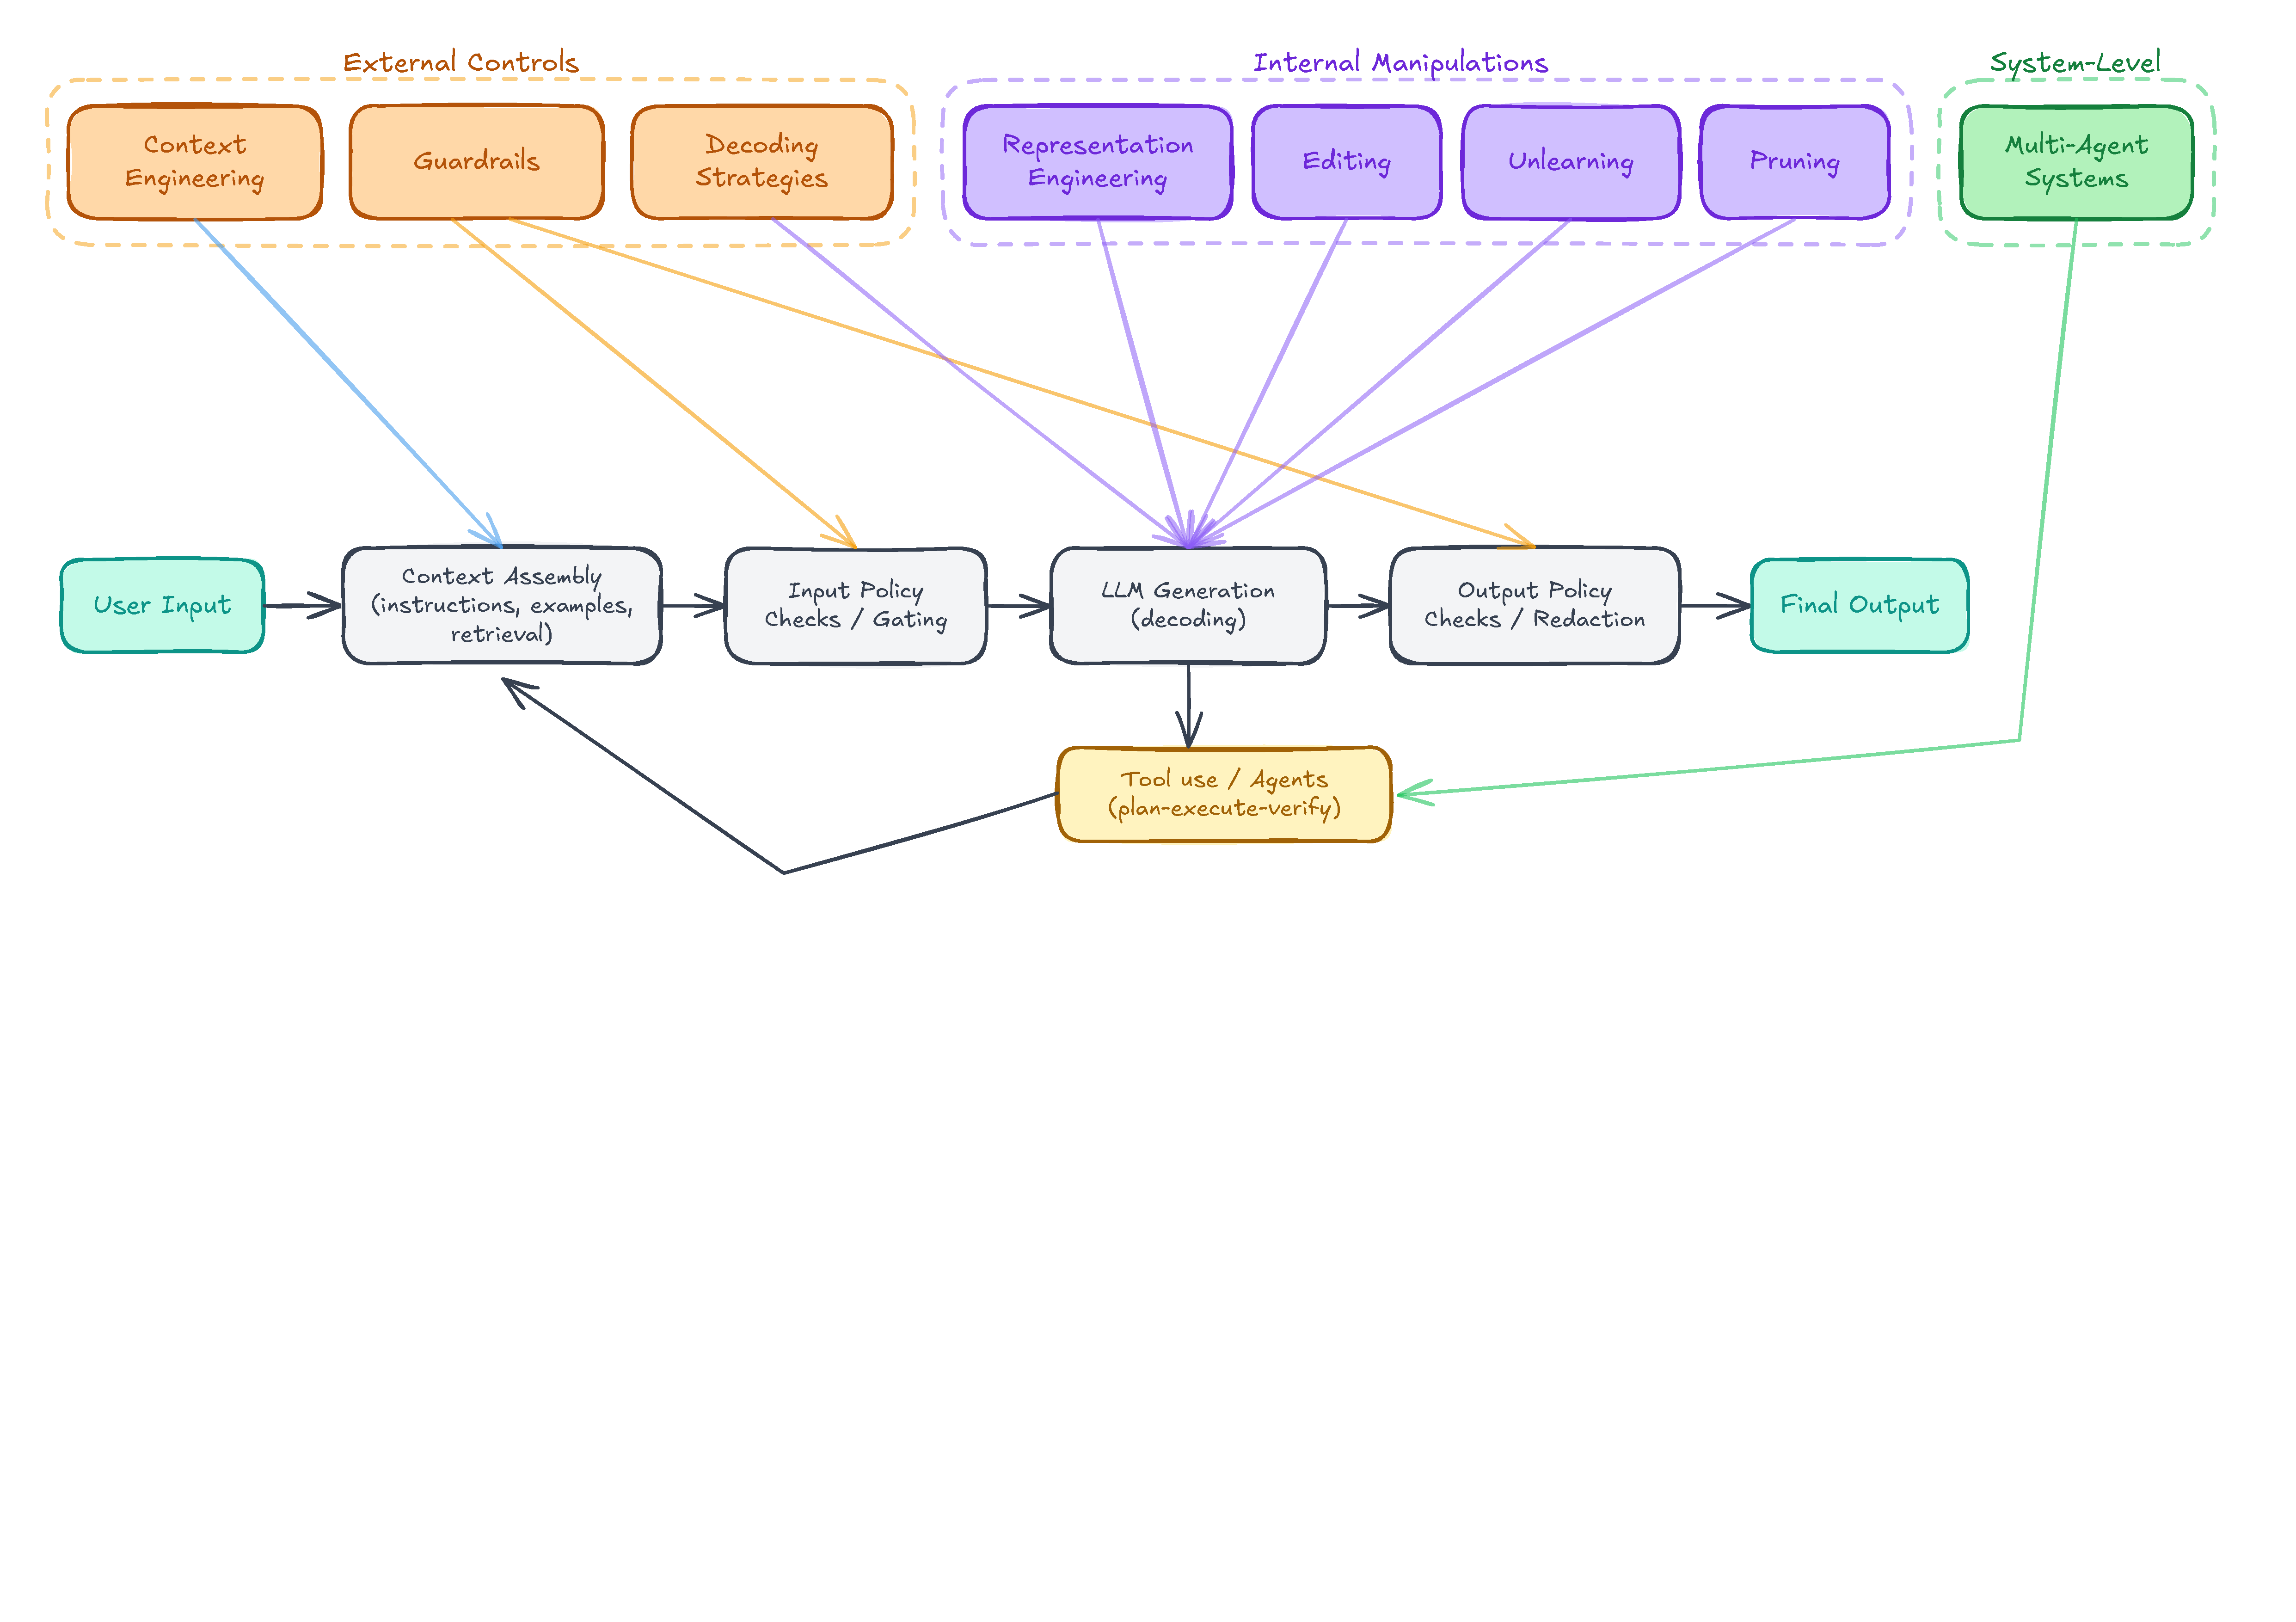
\includegraphics[width=1\linewidth]{figures/taxonomy_pipeline.pdf}
  \caption{TODO}
  \label{fig:taxonomy_pipeline}
\end{figure}

\begin{figure}[htbp]
  \centering
  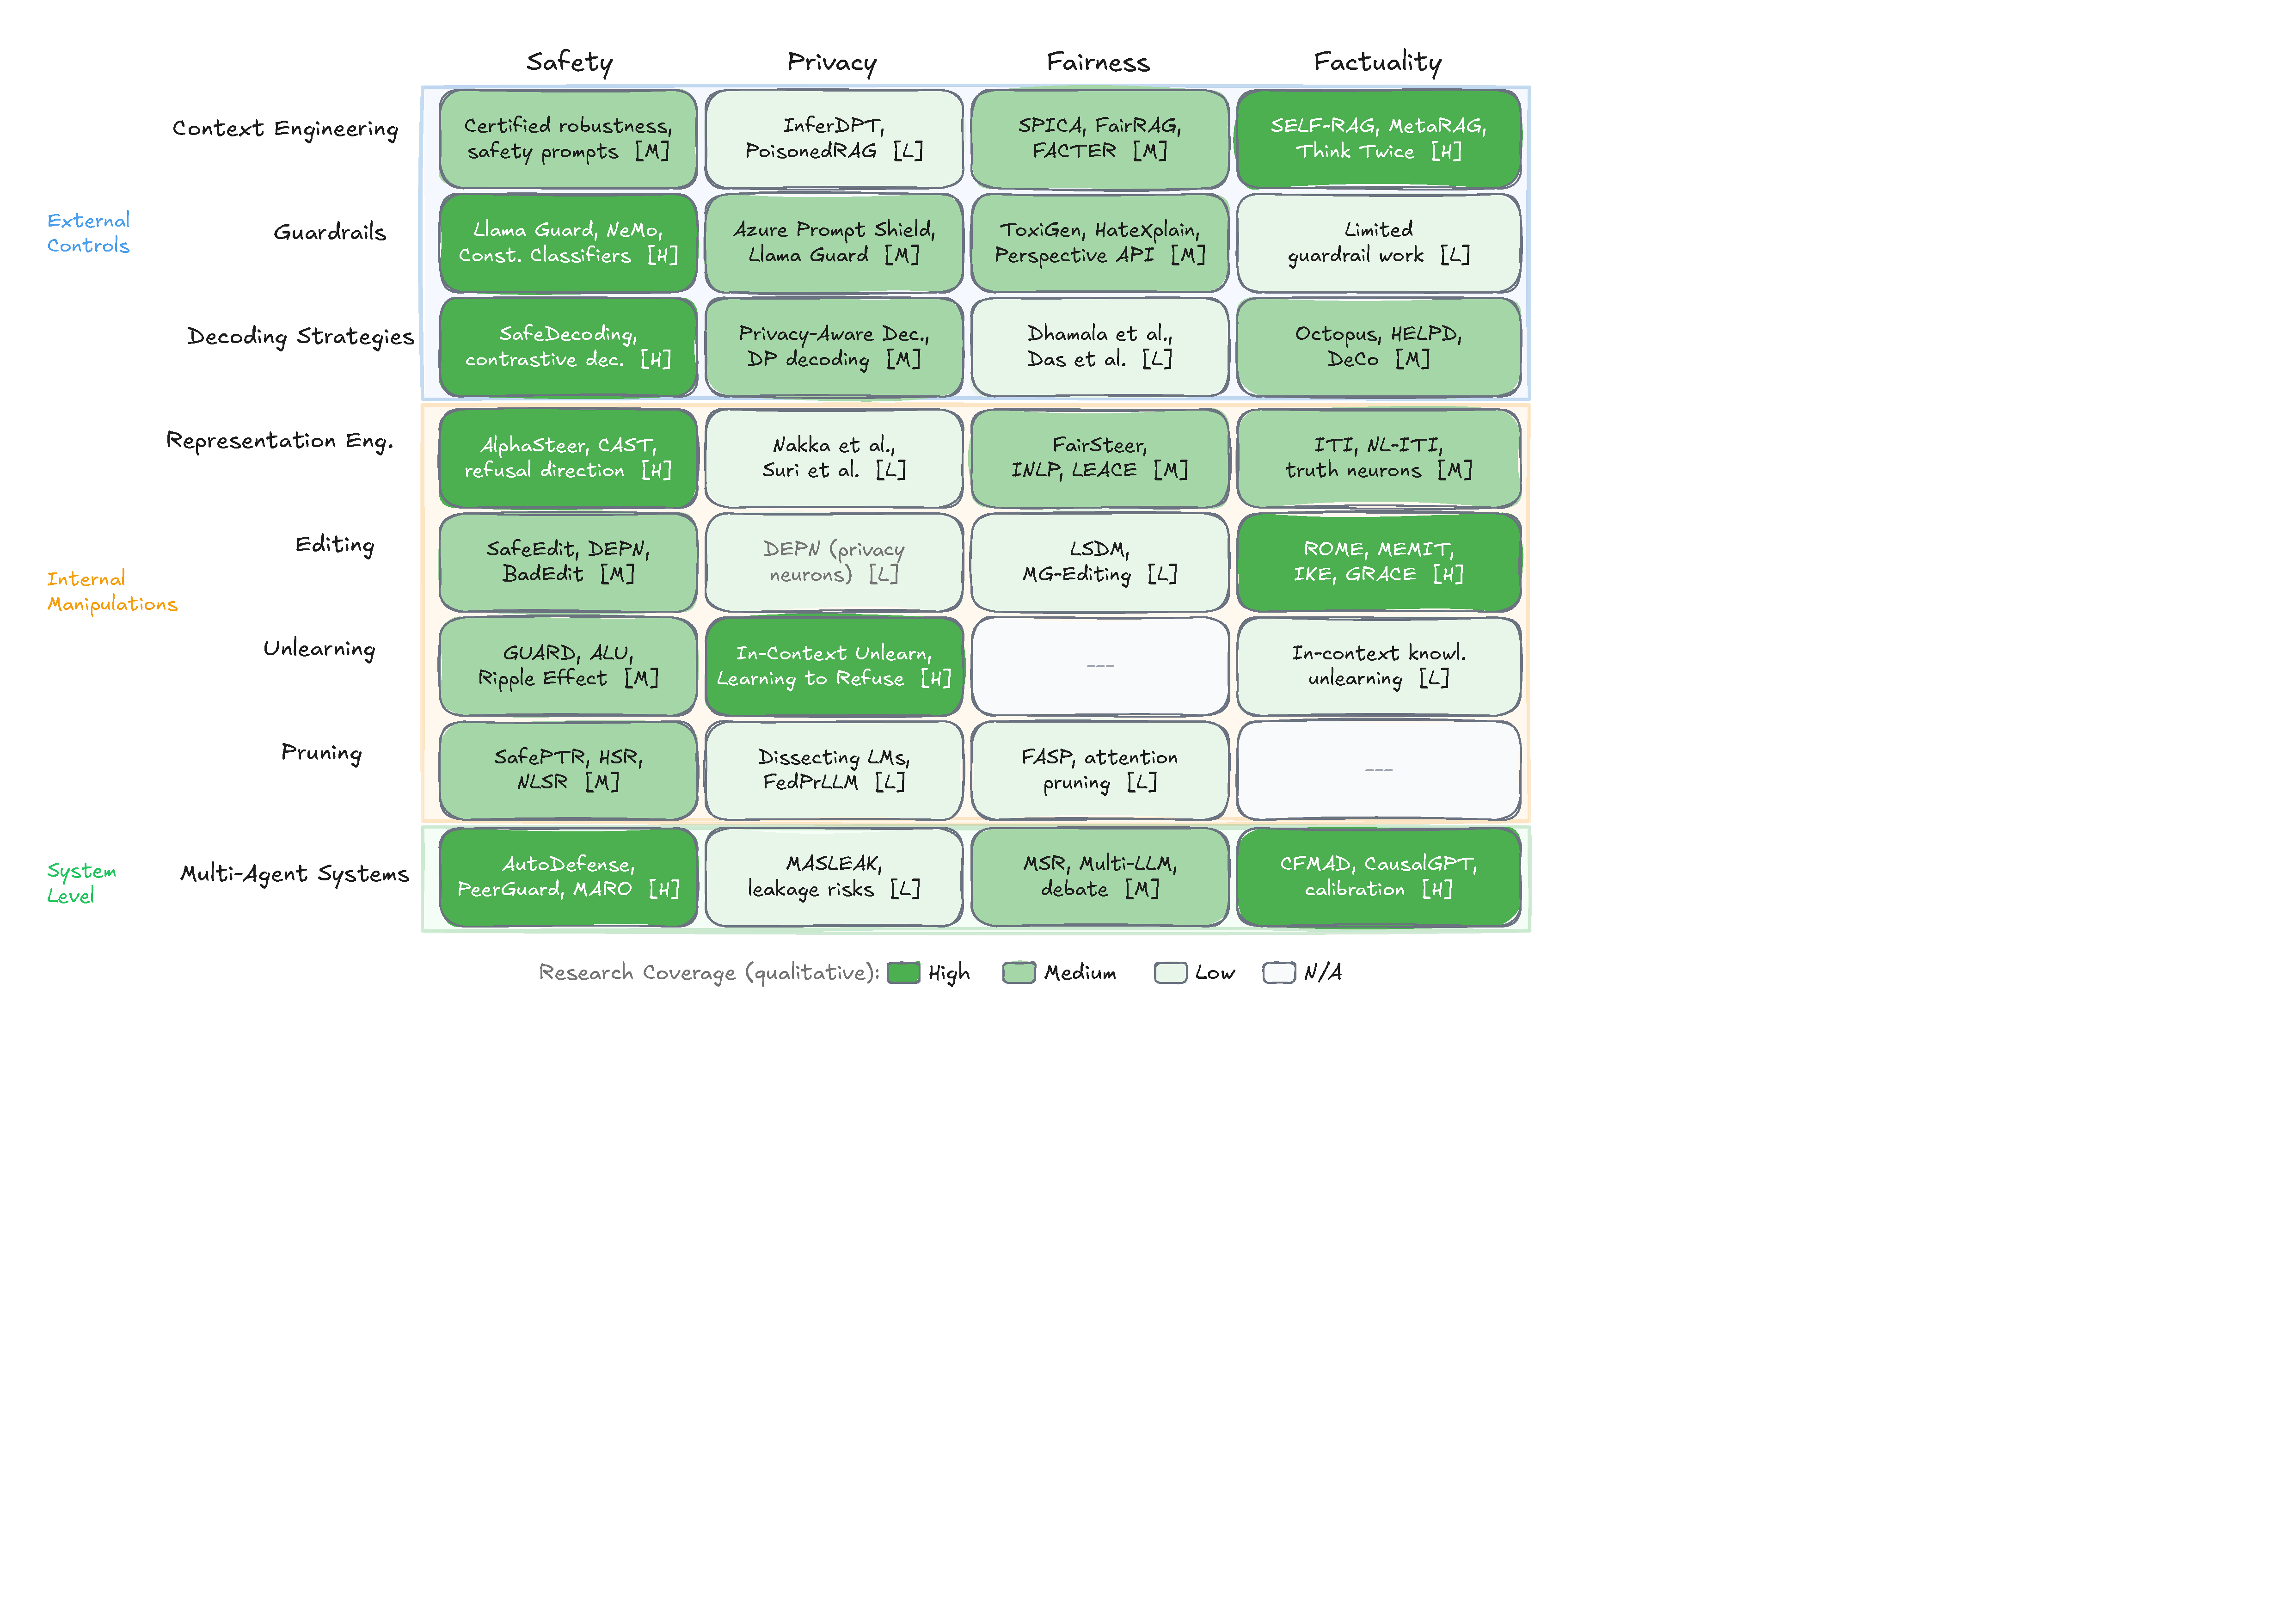
\includegraphics[width=1\linewidth]{figures/taxonomy_heatmap.pdf}
  \caption{TODO}
  \label{fig:taxonomy_heatmap}
\end{figure}

Large Language Models (LLMs) have rapidly evolved from experimental prototypes into widely deployed systems across domains such as healthcare, law, and finance. Built on massive neural architectures and trained over web-scale corpora, they demonstrate remarkable abilities in language understanding, generation, and reasoning. Yet, their growing role in sensitive decision-making introduces pressing concerns about trust. LLMs can produce misleading, biased, or harmful content, expose private information, or assert falsehoods with high confidence. In this survey, we focus on trustworthiness—a model’s consistent and reliable behavior. While alignment during training is essential, we argue that ensuring trustworthy behavior at deployment time also requires mechanisms that operate during inference.

Training methods such as instruction tuning and Reinforcement Learning from Human Feedback (RLHF) have been central to shaping the high-level behavior of LLMs. By modifying model parameters before deployment, these methods embed broad behavioral priors that guide how models respond to diverse inputs. However, once trained, updating a model’s behavior is often expensive, slow, or even infeasible, particularly when users have only API access or limited control over model weights. Meanwhile, real-world deployments demand frequent adaptation: organizations must revise safety policies, address emerging threats, and comply with evolving regulations. These realities highlight the need for a complementary approach. Inference-time methods provide a practical control layer for adapting model behavior after deployment. They are typically lightweight, modular, and do not require retraining, making them well-suited to dynamic, context-specific requirements.

Many inference-time techniques were originally developed to optimize model performance—reducing latency, improving fluency, or grounding responses through retrieval. More recently, these methods have been redirected toward a different objective: enforcing trustworthy behavior during generation. Beyond enhancing surface-level quality, they now serve as mechanisms for preventing harm, protecting privacy, and aligning model outputs with specific social or organizational expectations.

Static alignment methods, while foundational, are not equipped to meet the fluid demands of real-world deployment. Once trained, models are difficult to update, and retraining cycles are often too slow or costly to address urgent needs. In contrast, inference-time interventions can respond immediately to emerging requirements, such as (i) updating safety or content policies on short notice, (ii) tailoring behavior to specific users, jurisdictions, or applications, (iii) applying transparent interventions such as redaction or filtering for regulatory oversight, and (iv) mitigating newly discovered vulnerabilities, distribution shifts, or adversarial exploits. In these cases, the ability to steer or constrain model behavior without modifying its weights is essential. Inference-time methods provide this flexibility, acting as a dynamic counterpart to static training-time alignment and enabling reliable behavior under evolving conditions.

We define trustworthiness along four key dimensions: safety, the prevention of harmful, biased, or malicious outputs and the defense against misuse or jailbreaks; privacy, the avoidance of training data leakage and the protection of user inputs during inference; fairness, the reduction of systematic disadvantages to individuals or groups; and factuality, the grounding of outputs in verifiable knowledge to minimize hallucination.

Inference-time methods encompass a diverse and rapidly expanding set of techniques. To organize this landscape, we propose a taxonomy that categorizes approaches not by trust objective (e.g., safety or fairness), but by the mechanism of behavioral control they implement. This functional perspective highlights shared design patterns across seemingly disparate methods and clarifies trade-offs in granularity, invasiveness, and modularity. Rather than viewing these tools as isolated fixes, we present them as elements of a coherent design space for runtime trustworthiness interventions.

Our taxonomy comprises eight categories: Context Engineering, Guardrails, Decoding Strategies, Representation Engineering, Editing, Unlearning, Pruning, and Multi-Agent Systems. The goal is to frame these techniques as a principled, dynamic, and modular toolkit for inference-time control—capable of operating at varying levels of granularity and invasiveness.

\begin{itemize}
\item Context Engineering: Strategic prompt design through rules, instructions, or few-shot exemplars to guide outputs without modifying model parameters.
\item Guardrails: External modules that inspect inputs or outputs against safety or policy constraints, blocking, redacting, or regenerating content when violations occur.
\item Decoding Strategies: Manipulation of token-level distributions during generation to promote desired attributes (e.g., lower toxicity) or suppress undesired ones.
\item Representation Engineering (Steering): Direct modification of internal activations by adding or subtracting steering vectors associated with specific concepts (e.g., honesty).
\item Editing: Localized parameter updates to correct facts, update knowledge, or remove harmful associations efficiently.
\item Unlearning: Targeted removal of information, behaviors, or biases from a pre-trained model to fulfill data-forgetting requirements or disable harmful capabilities.
\item Pruning: Post-training removal of weights, neurons, or attention heads—originally for efficiency, now increasingly explored for its trust-related effects.
\item Multi-Agent Systems: Replacing single-model control with coordinated agent interactions such as debate or cross-verification, allowing reliability to emerge through collaboration.
\end{itemize}

By synthesizing these developments, this survey establishes a unified conceptual framework for inference-time trustworthiness. We map the current landscape, identify synergies across methods, examine trade-offs, and outline a research agenda for building reliably aligned systems under real-world deployment constraints.

\subsection{Related Surveys}
Our work sits at the intersection of three strands: inference efficiency, post-training capability enhancement, and broad-spectrum trustworthiness.

\paragraph{Efficiency-focused Surveys.}
Comprehensive surveys review inference-time optimizations such as quantization, distillation, and speculative decoding\citep{survey:inference_efficiency1}. Others target specialized settings like Mixture-of-Experts\citep{survey:inference_moe} or memory-footprint reduction for large deployments\citep{survey:inference_efficiency2}. These studies are foundational for understanding mechanics and cost, but their primary objective is computational performance rather than the explicit control of trustworthy behavior.

\paragraph{Surveys on Post-Training Capability Enhancement.}
A second line examines methods applied after pre-training to improve complex-task performance, including prompting-based techniques and reinforcement learning advances\citep{survey:post-training1, survey:post-training2}. The focus is to make models more capable reasoners or tool users. Alignment is peripheral; fine-grained enforcement of safety, privacy, or fairness at deployment is not the central goal.

\paragraph{Trustworthy-focused Surveys.}
Holistic surveys chart the landscape of trustworthy LLMs from data integrity to evaluation\citep{survey:trustworthy1, survey:trustworthy2}. Other work dives deep into specific facets—mitigating social bias in text-to-image generation\citep{survey:trustworthy_text2img}, safety for autonomous LLM agents\citep{survey:trustworthy_agents}, or machine unlearning\citep{survey:unlearning1, survey:unlearning2}. While invaluable, these efforts either organize by harm type or by a single solution family. To our knowledge, none provides a systematic, unified taxonomy that treats \emph{inference-time methods as a control plane} for trustworthiness across safety, privacy, fairness, and factuality.

\subsection{Contributions and Organization}
This survey analyzes inference-time methods for enhancing the trustworthiness of LLMs. Our primary contribution is a unified taxonomy that organizes post-hoc control techniques into eight categories, structured from external controls to internal manipulations—Context Engineering, Guardrails, Decoding Strategies, Representation Engineering, Editing, Unlearning, Pruning, and Multi-Agent Systems—and evaluates them against four deployment-critical dimensions: Safety, Privacy, Fairness, and Factuality.

Our key contributions are as follows:

\begin{itemize}
    \item \textbf{A Unified Taxonomy of Inference-Time Methods for Trustworthiness.} We organize eight categories of inference-time control into a coherent control-plane perspective that spans external, internal, and systemic interventions for deployed LLMs.
    \item \textbf{Systematic Cross-Dimensional Analysis.} We analyze how each category addresses Safety, Privacy, Fairness, and Factuality, clarifying capabilities, limitations, and trade-offs under deployment constraints.
    \item \textbf{Future Directions and Open Challenges.} We synthesize open problems on scalability, evaluation, and composition, and outline a research agenda for robustly aligned, real-world systems.
\end{itemize}

The remainder of the survey is organized as follows. \textbf{Sections \ref{sec:context_engineering}–\ref{sec:multi_agent_systems}} present the eight categories in our taxonomy and provide the cross-dimensional analysis, addressing our first and second contributions. \textbf{Section \ref{sec:evaluation}} then provides a critical analysis of evaluation benchmarks and trade-offs. \textbf{Section \ref{sec:challenges}} consolidates open challenges and future directions. \textbf{Section \ref{sec:conclusion}} concludes the survey.
